%PAGINA 1
\begin{frame}
    \frametitle{Arquitectura del Sistema}

    \begin{figure}[H]
        \centering
        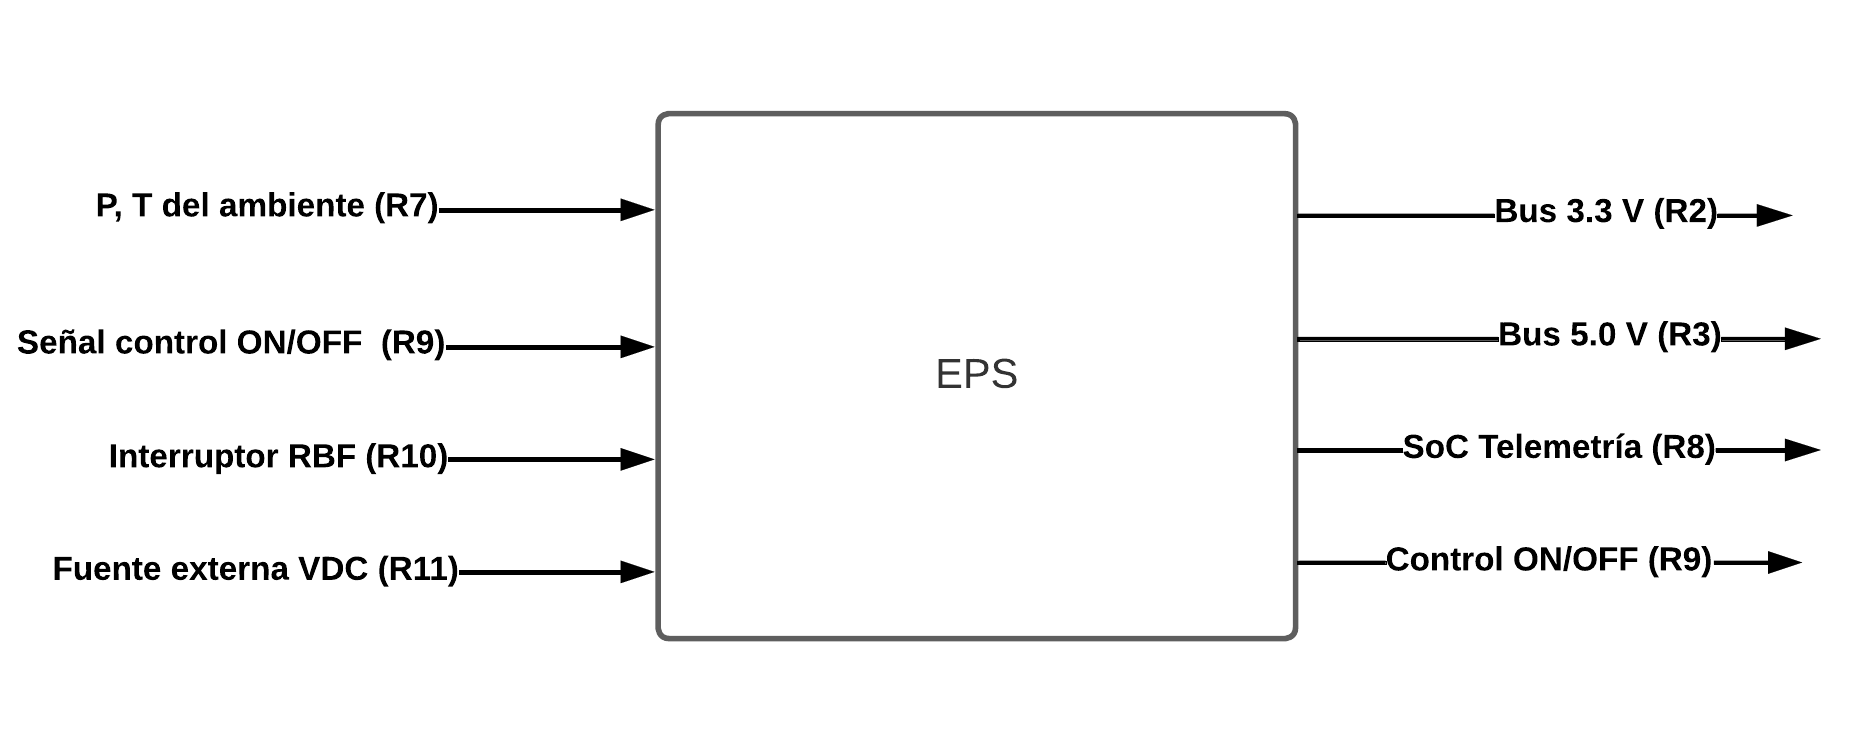
\includegraphics[width=\textwidth]{Level0.png} % Ajusta el tamaño según sea necesario
        \mycaption{Diagrama funcional nivel 0}
        \label{fig:level0DF}
    \end{figure}
\end{frame}

%PAGINA 2
\begin{frame}
    \frametitle{Arquitectura del Sistema}
    \begin{figure}[H]
        \centering
        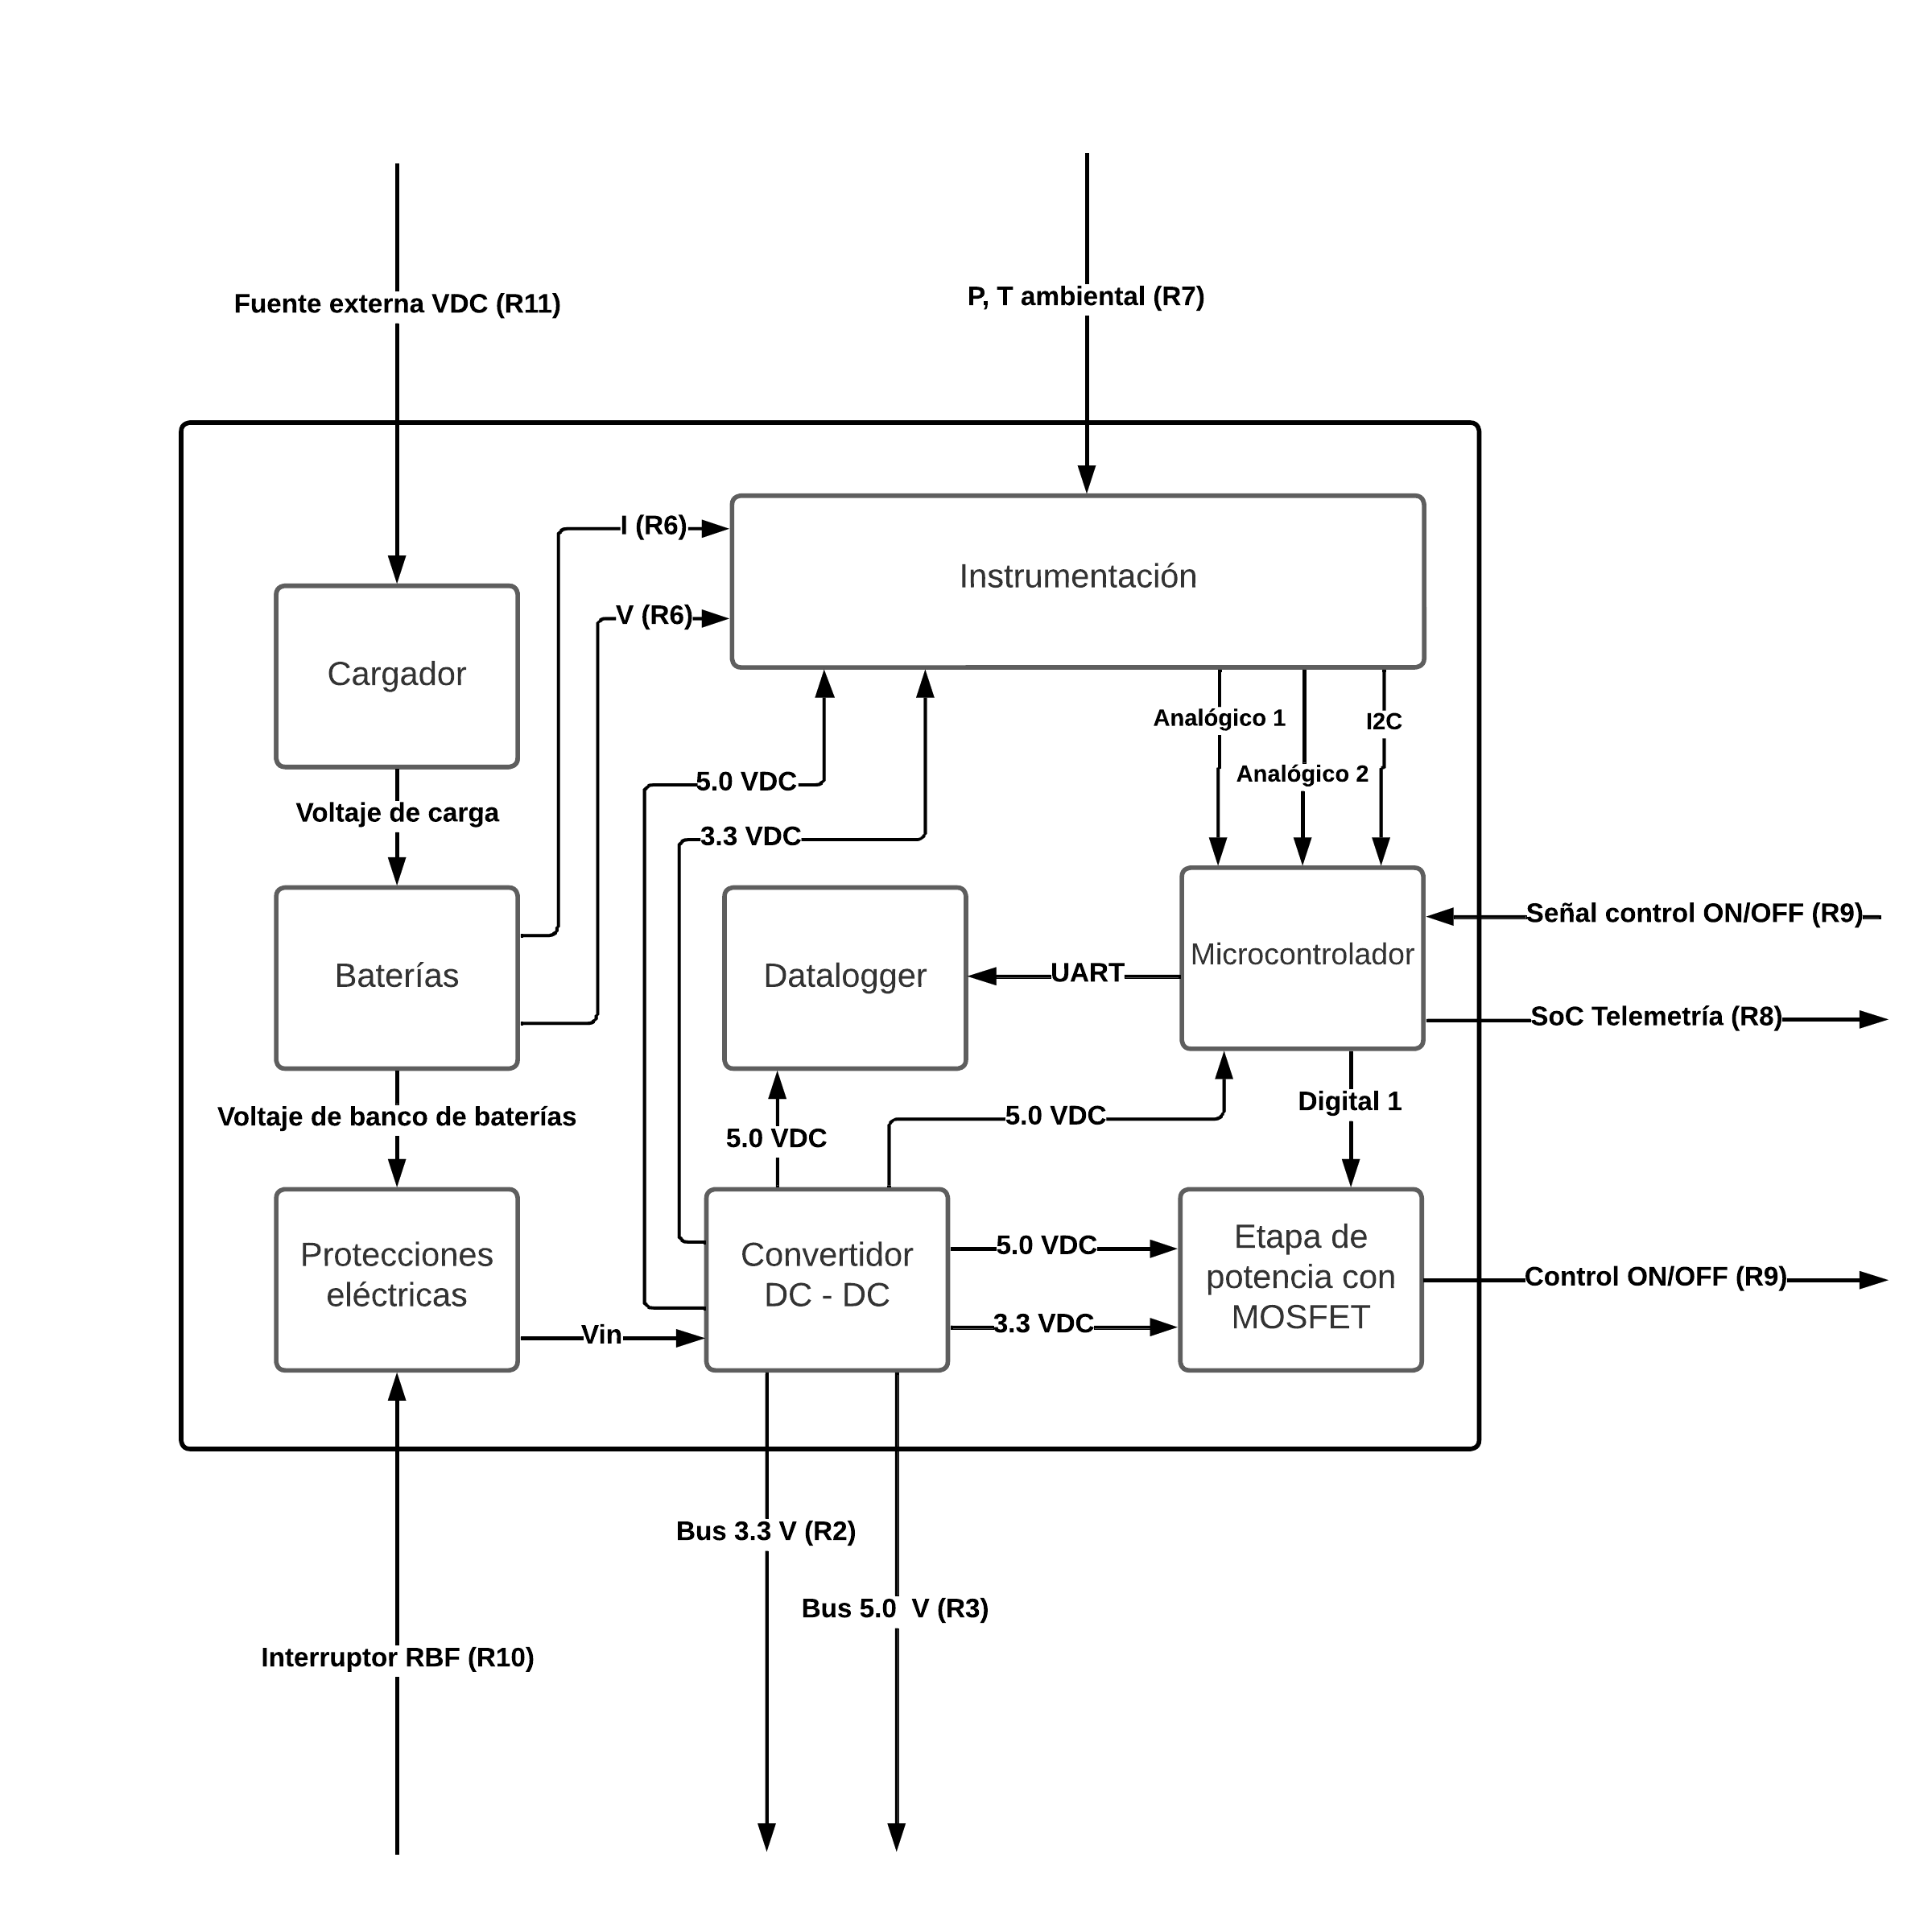
\includegraphics[width=0.60\textwidth]{Level1.png} % Ajusta el tamaño según sea necesario
        \mycaption{Diagrama funcional nivel 1}
        \label{fig:level0DF}
    \end{figure}
\end{frame}

%PAGINA 3
\begin{frame}
    \frametitle{Arquitectura del Sistema}

    \begin{figure}[H]
        \centering
        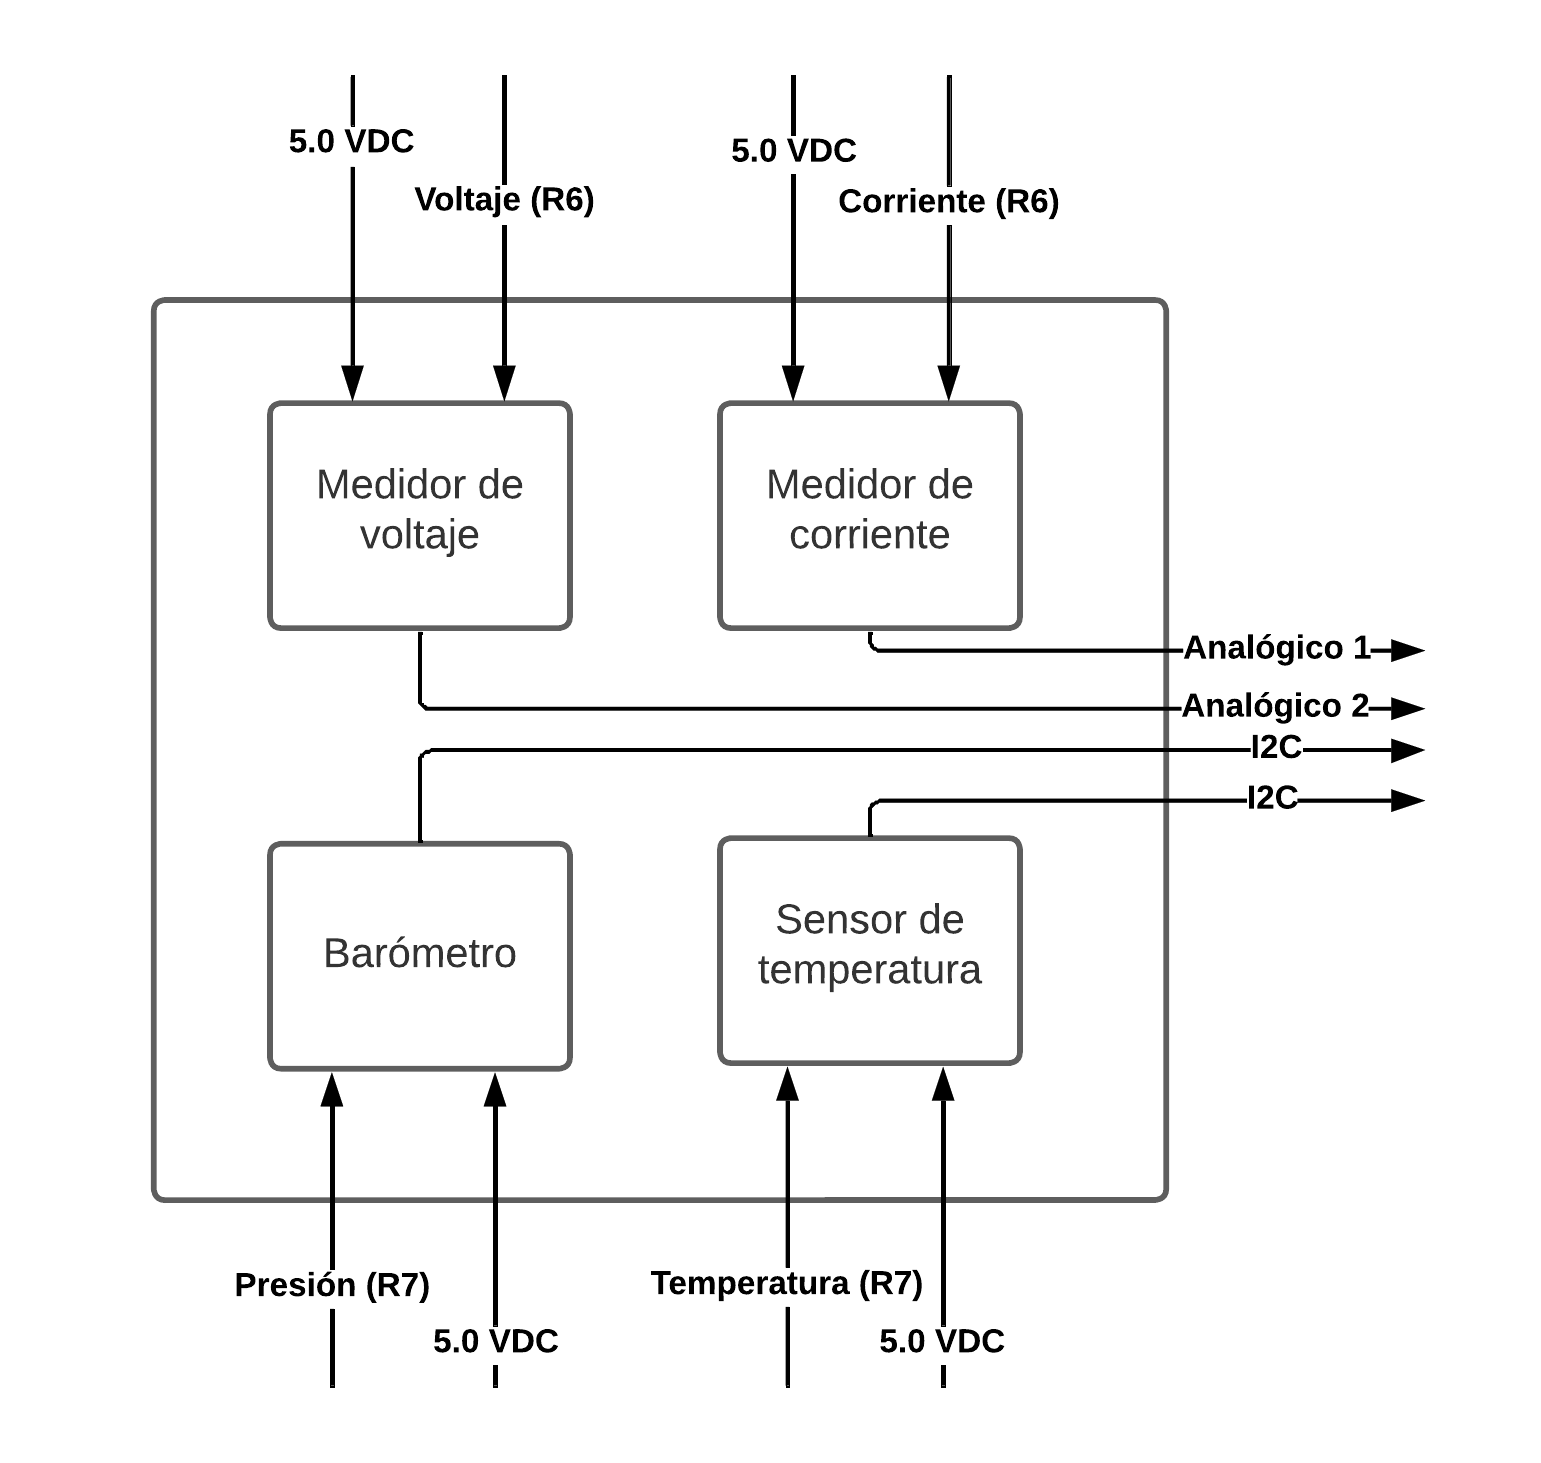
\includegraphics[width=0.6\textwidth]{Level2A.png} % Ajusta el tamaño según sea necesario
        \mycaption{Diagrama funcional nivel 2}
        \label{fig:level0DF}
    \end{figure}
\end{frame}


